% -*- mode: fundamental -*-

% ****************************************************************

\chapter{{\BSV}: Finite State Machines (FSMs) using {\tt StmtFSM}}

\markboth{Ch \arabic{chapter}: {\BSV}: FSMs}{\copyrightnotice}

\setcounter{page}{1}
% \renewcommand{\thepage}{\arabic{page}}
\renewcommand{\thepage}{\arabic{chapter}-\arabic{page}}

\label{ch_FSMs}

% ****************************************************************

\section{Introduction}

\index[BSV]{FSMs}
\index[BSV]{Finite State Machines}

So far, we have only been discussing pure combinational functions, for
which there is no concept of time.  Combinational functions are just
pure mathematical functions, ``instantaneously'' transforming input
values to output values.  In actual combinational circuits, there is
of course a finite delay through wires and gates, as dictated by
physics, but in the digital abstraction of time we think of this as
instantaneous.

However, a CPU, as shown in Figure~\ref{Fig_FSMs_Simple_Instr_Exec}
\begin{figure}[htbp]
% OLD \centerline{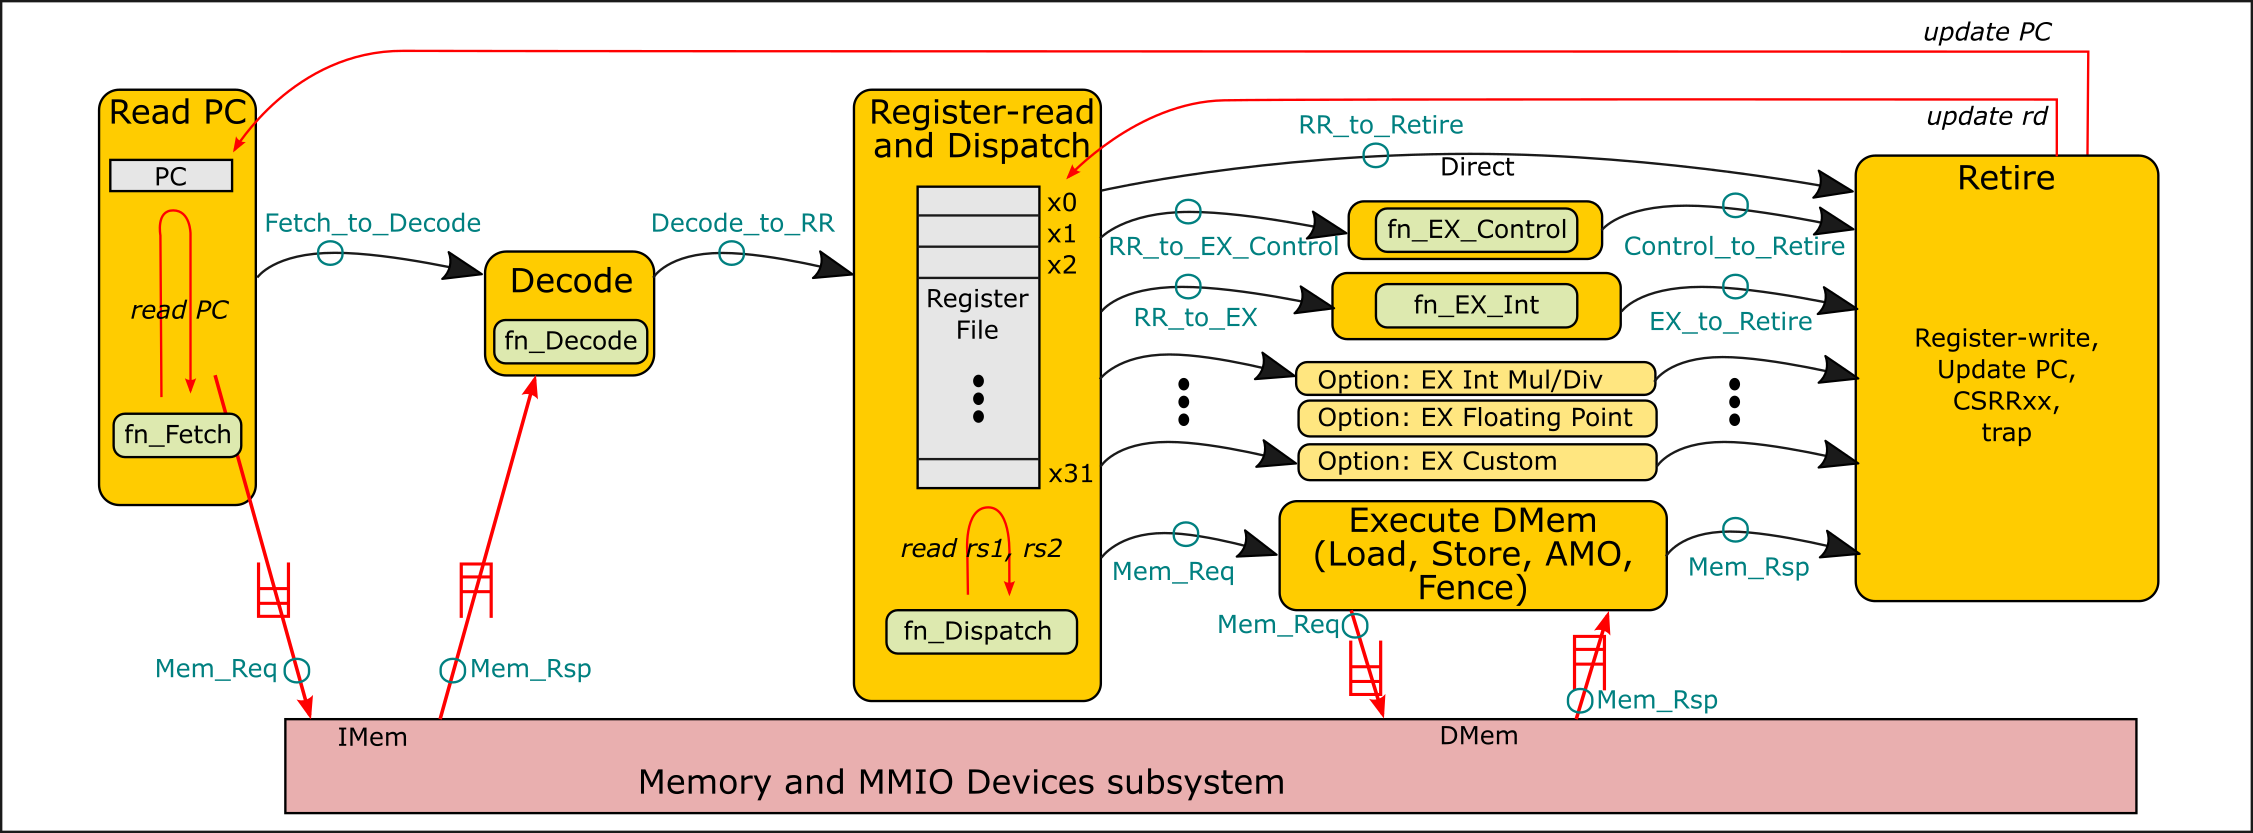
\includegraphics[width=6in,angle=0]{Figures/Fig_Instr_Exec_w_structs}}
  \centerline{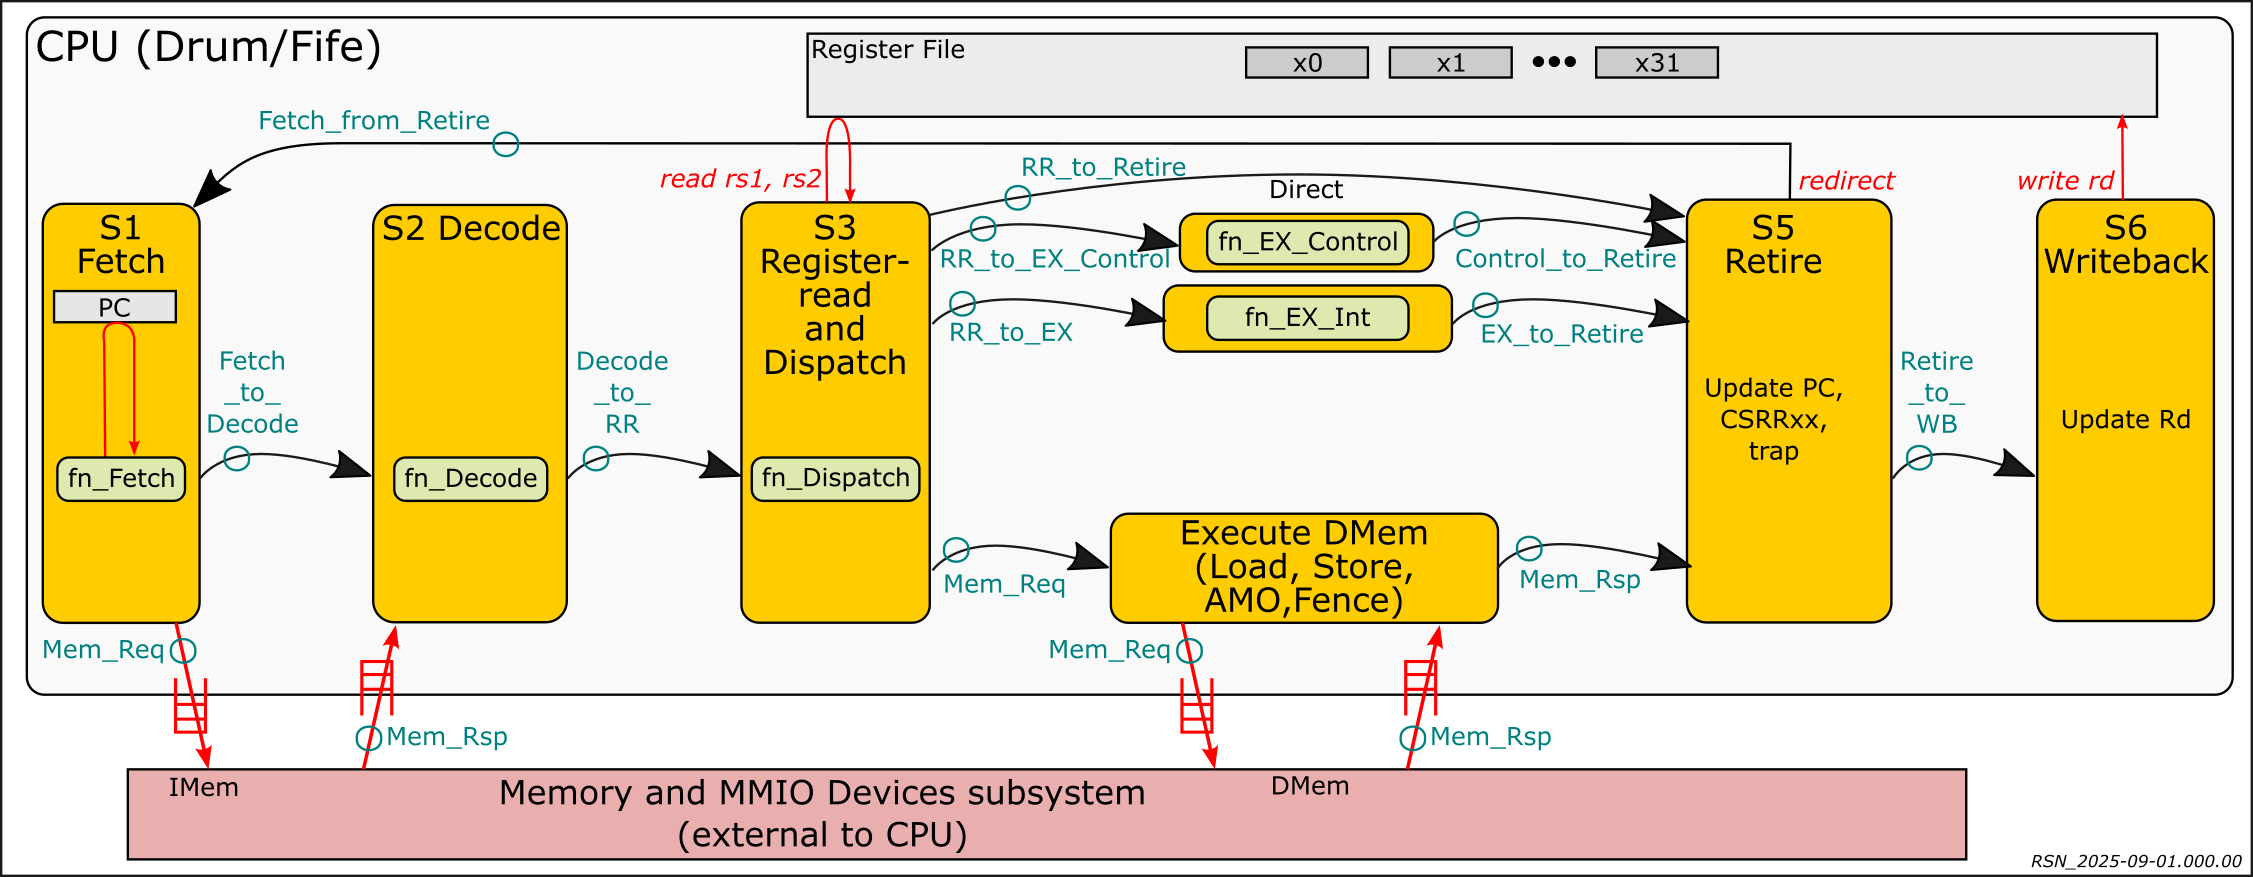
\includegraphics[width=6in,angle=0]{Figures/RSN_2025-09-01.000.00_FifeDrum_Stages_Multilayer_L1_L3}}
  \caption{\label{Fig_FSMs_Simple_Instr_Exec}
           Simple interpretation of RISC-V instructions
	   (same as Fig.~\ref{Fig_Simple_Instr_Exec_w_structs})}
\end{figure}
represents a \emph{processs}, a behavior that evolves over time.  For
example the {\DRUM} CPU executes one full instruction after another,
repeating forever the flow along the black arrows in the diagram. For
each instruction, first it performs a Fetch operation, which sends a
request to memory. Some time later, the memory sends back a response,
which is then processed by the Decode stage,
Register-Read-and-Dispatch stage and then one of the Execute stages.
The Execute DMem stage sends a request to memory. Some time later, the
memory sends back a response, which is processed in the Retire stage.
Finally, the process loops back to the Fetch stage, and repeats for
the next instruction.

The simplest temporal process in hardware systems is the \emph{FSM}
(Finite State Machine).  A classical notation for FSMs is the
so-called ``bubble-and-arrow'' diagram.
Figure~\ref{Fig_FSM_Bubble_and_Arrow} shows a greatly over-simplified
bubble-and-arrow diagram for an FSM controlling an elevator (a lift).
\begin{figure}[htbp]
  \centerline{\includegraphics[width=6in,angle=0]{Figures/Fig_FSM_Bubble_and_Arrow}}
  \caption{\label{Fig_FSM_Bubble_and_Arrow}
           A (greatly over-simplified) FSM for controlling an elevator.}
\end{figure}
Each bubble represents a distinct \emph{state} of the system, and the
arrows connecting bubbles represent \emph{transitions} between states.
Transitions are typically enabled by some boolean condition on the
current state, and/or availability of some particular input from the
environment (``{\bf C:}'' in the diagram).  A transition moves the
system to another state, and may perform some action, including
producing some output to the environment (``{\bf A:}'' in the
diagram).  In bubble-and-arrow diagrams, each arrow is often labeled
with the condition that enables the transition, and by any actions
performed by the transition.

\index[BSV]{Drum!as an FSM}

Figure~\ref{Fig_FSMs_Simple_Instr_Exec} can be interpreted as a
bubble-and-arrow FSM diagram: each yellow rectangle (bubble) is a
state, and the process transitions from state to state, thereby
executing RISC-V instructions.  This is exactly what the {\DRUM} CPU
does.  In Figure~\ref{Fig_FSMs_Simple_Instr_Exec} the arrows are
labeled by the information (a struct) that is produced in one state
and consumed by another.

In this chapter we describe some special constructs for FSMs in {\BSV}.
In the next chapter we will discuss using these FSM constructs to code
the {\DRUM} CPU.

% ----------------
\vspace{2ex}

NOTE: \fbox{\footnotesize
\begin{minipage}{0.9\textwidth}

In the literature one may read about FSMs where, from some state, we
could have a choice of transitions to different destination states.
These are called \emph{non-deterministic} FSMs.  In our designs we are
only concerned with \emph{deterministic} FSMs where the conditions on
the arrows emerging from a state are mutually exclusive, so that they
always identify a unique possible next state.

\end{minipage}}
% ----------------

% ================================================================

\subsection{Sequential FSMs, Concurrent FSMs, and Digital Hardware}

\index[BSV]{FSMs!sequential {\vs.} concurrent}
\index[BSV]{FSMs!concurrent {\vs.} sequential}

Classical FSMs in the literature are \emph{sequential} FSMs---every
transition is from the current state to a unique, particular next
state.\footnote{Even in non-deterministic FSMs, though there may be
several possible next-states, exactly one next-state is
non-deterministically chosen.}

Any digital system (including an entire computer) can theoretically be
viewed as a single (possibly giant!) FSM.  The current-state is the
current collective state of every register bit and every memory bit in
the system.  State transitions depend on the current state and any
external inputs.  Although theoretically correct, this is an
impractical, non-scalable, and not very useful way of viewing complex
digital systems.

Most non-trivial digital hardware systems are better viewed as
composed of multiple \emph{concurrent, communicating FSMs}, {\ie}
multiple classical FSMs running concurrently and independently and
communicating with each other (an output from one FSM may be an input
to another FSM).  Figure~\ref{Fig_FSMs_Concurrent} sketches the idea.
\begin{figure}[htbp]
  \centerline{\includegraphics[width=6in,angle=0]{Figures/Fig_FSMs_Concurrent}}
  \caption{\label{Fig_FSMs_Concurrent}
           \begin{minipage}[t]{0.75\textwidth}
           Concurrent, independent FSMs. \\
	   The grey arrows indicate communication {\via} registers, FIFOs, ...
	   \end{minipage}}
\end{figure}
Different {\BSV} module instances are separate FSMs, each running
their own process(es).  These separate FSMs may communicate with each
other {\via} shared state (registers, FIFOs, register files, {\etc}).
This is a more \emph{modular} and \emph{scalable} way to think about
complex digital systems.

\index[BSV]{Drum!as an FSM concurrent with its memory system}

{\DRUM} CPU execution is a sequential FSM, but the overall system in
which {\DRUM} is embedded can be viewed as a pair of concurrent FSMs:
{\DRUM} and the Memory System (see Figure~\ref{Fig_CPU_Simulation}).
Each has its own internal FSM process and behavior, and they
communicate memory requests and responses back and forth.

\index[BSV]{Fife!as a set of concurrent FSMs}

For {\FIFE}, we will interpret \emph{each} yellow box in
Figure~\ref{Fig_FSMs_Simple_Instr_Exec} as its own FSM.  All these
FSMs run concurrently (and concurrently with the memory system), and
communicate various struct values (labels in
Figure~\ref{Fig_FSMs_Simple_Instr_Exec}) through FIFOs between the
FSMs.

% ================================================================

\subsection{Communicating between FSM states and between concurrent FSMs}

\index[BSV]{FSMs!communication between states}
\index[BSV]{FSMs!communication between concurrent FSMS}

In a sequential FSM, communication between states is easily
accomplished using ordinary registers---one transition writes into a
register, and another transition reads from the register.  Because the
FSM is sequential, transitions occur in some well-defined order, and
so there is a well-defined order in which the register is written and
read.

Communication between concurrent FSMs, on the other hand is more
easily accomplished using FIFOs.  Concurrent FSMs may run at different
rates and so there may not be any predictable temporal ordering
between when FSM A produces a datum and when another FSM B tries to
consume the datum.  Instead, we let FSM A \emph{enqueue} the datum
into a FIFO, and let FSM B \emph{dequeue} the datum from the FIFO.  If
FSM B tried to consume the datum before it has been produced, it will
simply ``block'', or stall, trying to read an empty FIFO, until FSM A
produces the datum into the FIFO.

FIFOs between concurrent FSMs also enables \emph{pipelining} or
\emph{streaming}.  FSM A can repeatedly enqueue data into a FIFO even
if FSM B is not yet ready to consume it.  FSM B can repeatedly consume
data already produced by FSM A.  If the FIFO becomes full, FSM A will
simply block when it tries to enqueue the next datum into it.  If the
FIFO becomes empty, FSM B will simply block until data is available.
The FIFO is said to perform automatic ``flow control'' between
producer and consumer FSMs.  In this way, communication via FIFOs
between concurrent FSMs is more ``elastic'', or ``asynchronous''.

In {\DRUM}, where Figure~\ref{Fig_FSMs_Simple_Instr_Exec} represents
the states (yellow bubbles) and transitions (black arrows) of a
sequential FSM, we will use registers to communicate between states.
We use FIFOs to communicate to/from the concurrent external FSM, the
memory system.

In {\FIFE}, where the yellow bubbles of
Figure~\ref{Fig_FSMs_Simple_Instr_Exec} represent concurrent FSMs, we
will use FIFOs to communicate between the FSMs.

% ****************************************************************

\section{{\tt StmtFSM}: structured FSM processes in {\BSV}}

\label{Sec_Rules_StmtFSM}
\label{Sec_StmtFSM}

\index[BSV]{rule}
\index[BSV]{StmtFSM@{\tt StmtFSM}!an abtstraction of rules}
\index[BSV]{StmtFSM@{\tt StmtFSM}!structured process}

The fundamental behavioral/temporal primitive in {\BSV}, to specify
processes, is the \emph{rule} but we will postpone a detailed
discussion of rules until Chapters~\ref{ch_Rules_I} and
\ref{ch_Rules_II}.  Rules can express arbitrary process flows, both
structured and unstructured.  {\BSV}'s \verb|StmtFSM| is a
higher-level notation that captures the idea of certain
\emph{structured} processes (rule execution flows).  \verb|StmtFSM| is
ultimately implemented (by the \emph{bsc} compiler) with rules, so it
does not add any fundamental semantic power to the language---anything
we write with {\tt StmtFSM} can also be written directly with rules.
Section~\ref{Sec_StmtFSM_vs_rules} discusses when to use
\verb|StmtFSM| and when to use rules.

\verb|StmtFSM| is a sub-language within {\BSV} for specifying
structured FSMs.  The sub-language which we use in {\DRUM} has the
following grammar (Section~\ref{Sec_StmtFSM_more_features}
describes more available features in {\tt StmtFSM}):

\hmm
\begin{tabular}{lcl}
{\tt Stmt}  & ::= & an {\tt Action} expression \\
            &  |  & a  sequence ({\tt seq} block) of {\tt Stmt}s \\
            &  |  & an if-then-else of two {\tt Stmt}s \hmm (conditionals)\\
            &  |  & a while-loop around a {\tt Stmt}
\end{tabular}

The basic primitive is an expression of type \verb|Action| (which
includes {\tt action}-{\tt endaction} blocks that may contain
sub-actions).  This specifies an FSM which just performs that action
once (the {\tt Action} expression becomes the body of a single {\BSV}
rule).  Then, we \emph{compose} larger FSMs from smaller FSMs by
nesting them in sequences, conditionals and
loops. Figure~\ref{Fig_FSMs_Structured} illustrates this
compositionality.
\begin{figure}[htbp]
  \centerline{\includegraphics[width=6in,angle=0]{Figures/Fig_FSMs_Structured}}
  \caption{\label{Fig_FSMs_Structured}
           Structured FSMs, built compositionally.}
\end{figure}
Every {\tt Stmt} has a single start state and single end state.  Note
that each composition scheme itself results in a {\tt Stmt} with a
single start and end state.  This allows them to be nested
recursively.

We will use these \verb|StmtFSM| constructs to code {\DRUM}, which is a
simple sequential process.  \verb|StmtFSM| will not be adequate to
code {\FIFE}, which is a collection of concurrent FSMs; for that, we will
use rules explicitly.

% ----------------
\vspace{2ex}

NOTE: \fbox{\footnotesize
\begin{minipage}{0.9\textwidth}

We have already encountered examples of sequential {\tt StmtFSM}s,
with just a sequential block, in the simple testbench in
Section~\ref{BSV_small_testbench} and in many of the testbenches in
the exercises so far.

\end{minipage}}
% ----------------

% ****************************************************************

\section{Actions and the {\tt Action} type}

\index[BSV]{Action@{\tt Action}!Type of actions}

The fundamental building-block for \verb|StmtFSM| is the ``action'',
which is a statement/expression of type \verb|Action|.  Some common
examples:

{\footnotesize
\begin{Verbatim}[frame=single, numbers=left]
   rg_pc <= rg_pc + 4;            // Assignment to a register
   f_Fetch_to_Decode.deq;         // Dequeue a fifo
   f_Decode_to_RR.enq (v);        // Enqueue into a fifo
   $display ("Hello, World!");    // Print something (in simulation only)
\end{Verbatim}
}

We discussed the \verb|Action| (and \verb|ActionValue|) types in
Section~\ref{Sec_Pure_vs_Side_Effect_functions}.  We used them in the
return type of the \verb|fn_Fetch| function in
Section~\ref{Sec_fn_Fetch}.  To recap, an expression with
\verb|Action| or \verb|ActionValue| type is one that potentially has a
side effect, as in each of the above example statements.

As discussed in Section~\ref{Sec_Register_syntactic_shorthands} the
first assignment statement is syntactic shorthand for:

{\footnotesize
\begin{Verbatim}[frame=single, numbers=left]
   rg_pc._write (rg_pc._read + 4)
\end{Verbatim}
}

{\ie} it is an invocation of the register \verb|_write| method which,
as described in
Section~\ref{Sec_Register_interface} has type
\verb|Action|.  Similarly, as described in
Section~\ref{Sec_FIFOF_interface}, fifo \verb|enq|
and \verb|deq| methods have return-type \verb|Action|, so the
statements \verb|f_D_to_RR.enq (v)| and \verb|f_D_to_RR.enq (v)| have
type \verb|Action|.

\index[BSV]{display@{\tt \$display} has {\tt Action} type}

\verb|$display()| is a built-in construct in {\BSV} that also has type
\verb|Action|.

% ================================================================

\subsection{{\tt Action} blocks: composing actions into larger actions}

\index[BSV]{Action@{\tt Action}!{\tt action}-{\tt endaction} blocks}

The \verb|Action| type is recursive: it is either a primitive action
(like those described above), or it is a collection of things of type
\verb|Action|, collected using an \verb|action| block (bracketed by
the {\BSV} keywords \verb|action| and \verb|endaction|).  For example the
above primitive actions can be collected into a single entity which
itself has type \verb|Action|:

{\footnotesize
\begin{Verbatim}[frame=single, numbers=left]
   action
      rg_pc <= rg_pc + 4;          // Assignment to a register
      f_F_to_D.deq;                // Dequeue a fifo
      f_D_to_RR.enq (v);           // Enqueue into a fifo
      $display ("Hello, World!");  // Print something (in simulation only)
   endaction
\end{Verbatim}
}

Although the actions in an \verb|action| block must be written in some
textual order, \verb|action| \emph{blocks do not involve any temporal
sequencing.}  There is no temporal ordering of the actions in an
\verb|action| block.  All the actions in an \verb|action| block
(either directly in the block or, recursively in a sub-block) occur
``instantly'' and ``simultaneously''.  Referring to
Section~\ref{Sec_Interface_HW}, in hardware the ENABLE signals of all
actions in an \verb|action| block are asserted simultaneously.  In the
example above, lines 2-5 could have been written in any order with no
change in meaning/behavior.

% ================================================================

\subsection{Binding names in {\tt Action} blocks}

\index[BSV]{let@{\tt let}!in {\tt Action} blocks}

It is often convenient to give a meaningful name to a sub-expression
in an {\tt Action} block.  For example:

{\footnotesize
\begin{Verbatim}[frame=single, numbers=left]
   action
      Bit #(XLEN) next_pc = rg_pc + 4;
      rg_pc <= next_pc;
      $display ("Next PC is %08h", next_pc);
   endaction
\end{Verbatim}
}

Here, we bind the identifier \verb|next_pc| in line 2, and then use it
in lines 3 and 4.  We can often replace the type in the binding with
the keyword {\tt let}, if the type is obvious from the context (the
\emph{bsc} compiler will figure it out):

{\footnotesize
\begin{Verbatim}[frame=single, numbers=left]
   action
      let next_pc = rg_pc + 4;
      rg_pc <= next_pc;
      $display ("Next PC is %08h", next_pc);
   endaction
\end{Verbatim}
}

The \emph{scope} of the identifier, {\ie} the region of program text
where it is available for use, are the remaining statements in the
{\tt Action} block (including inside any syntactically nested
statements).

A binding, per se, \emph{is not an action!}  It is just a convenience,
giving a name to the value of the right-hand side expression.

Bindings (whether with an explicit type or with \verb|let|) impose
some syntactic ordering on statements in the block: a binding of an
identifier must precede any use of that identifier.  In the previous
two examples, line 2 (the binding) must precede lines 3 and 4 (the
actions), but lines 3 and 4 could be written in the opposite order.
Note, this is not a \emph{temporal} sequencing; all actions in the
block still occur simultaneously.

% ****************************************************************

\section{{\tt StmtFSM}: sequences of actions}

\index[BSV]{StmtFSM@{\tt StmtFSM}!seq@{\tt seq .. endseq}: sequences of actions}

Our first construct that has temporal behavior is the
\verb|seq|-\verb|endseq| block.  Each item in the block is an entity
of type \verb|Action| or \verb|Stmt|, and they are performed
sequentially, one after another.

\begin{tabbing}
\hmm \= \hm \kill
\hmm \> {\tt seq} \\
     \> \hm    ... \emph{an} {\tt Action} \emph{or} {\tt Stmt} ... {\tt ;} \\
     \> \hm    ... \\
     \> \hm    ... \emph{an} {\tt Action} \emph{or} {\tt Stmt} ... {\tt ;} \\
     \> {\tt endseq}
\end{tabbing}

\index[BSV]{FSMs!Stmt@{\tt Stmt}: type of argument to FSM module constructors}

The entire \verb|seq| block itself has type \verb|Stmt|, and so it can
be nested inside other \verb|StmtFSM| constructs.

The testbench in Section~\ref{BSV_small_testbench} contains an example
of a \verb|seq| block.

% ****************************************************************

\section{{\tt StmtFSM}: conditionals (if-then-else)}

\index[BSV]{StmtFSM@{\tt StmtFSM}!if@{\tt if-then-else}: process conditional}
\index[BSV]{if-then-else!Ordinary expression \emph{vs} {\tt StmtFSM} process}

Conditional process execution can be expressed with traditional
if-then-else notation:

\begin{tabbing}
\hmm \= \hm \kill
\hmm \> {\tt if} \\
     \> \hm    ... \emph{an} {\tt Action} \emph{or} {\tt Stmt} ... \\
     \> {\tt else} \\
     \> \hm    ... \emph{an} {\tt Action} \emph{or} {\tt Stmt} ... \\
\end{tabbing}

The entire if-then-else construct itself has type \verb|Stmt|, and so
it can be nested inside other \verb|StmtFSM| constructs.

% ----------------
\vspace{2ex}

NOTE: \fbox{\footnotesize
\begin{minipage}{0.9\textwidth}

In Section~\ref{BSV_Combo_Circuits_if_then_else} we described ordinary
{\BSV} if-then-else expressions, which often represent hardware
multiplexers, where both arms are ``evaluated'' (the hardware exists
for both sides) and the multiplexer merely selects one of the two
outputs.

\vspace{1ex}

{\tt StmtFSM} uses the same notation, but here it represents a
\emph{process}, and only one of the two arms is executed (like
if-then-else in most software programming languages).

\vspace{1ex}

There is no ambiguity in these two uses of if-then-else notation---the
context always clearly distinguishes what we mean, because there is no
overlap between ordinary expressions and {\tt StmtFSM} constructions.

\end{minipage}}
% ----------------

% ****************************************************************

\section{{\tt StmtFSM}: while-loops}

\index[BSV]{StmtFSM@{\tt StmtFSM}!while@{\tt while}-loop repetition}

Repetitive processes can be expressed with traditional while-loop notation:

{\footnotesize
\begin{Verbatim}[frame=single, numbers=left]
   while (... Bool expression ...)
      ... expression of type Stmt ...
\end{Verbatim}
}

The entire while-loop construct itself has type \verb|Stmt|, and so it
can be nested inside other \verb|StmtFSM| constructs.

% ****************************************************************

\section{{\tt StmtFSM}: pausing until some condition holds}

\index[BSV]{StmtFSM@{\tt StmtFSM}!await@{\tt await}: pausing until some condition}

An action in a \verb|StmtFSM| can be the \verb|await(b)| action, which
simply waits until the boolean expression in its argument evaluates to
true:

{\footnotesize
\begin{Verbatim}[frame=single, numbers=left]
   await (... Bool expression ...);
\end{Verbatim}
}

Of course, because it is paused, the \verb|Stmt| containing an
\verb|await| cannot itself cause the value to change since it cannot
change any state that would affect the expression.  The state-change
thus has to be effected by some other part of the {\BSV} design (a
concurrent FSM, or a rule), not this particular \verb|Stmt|.

% ****************************************************************

\section{{\tt StmtFSM}: {\tt mkAutoFSM}: a simple FSM module constructor}

\label{Sec_AutoFSM}

\index[BSV]{StmtFSM@{\tt StmtFSM}!{\tt mkAutoFSM} module}
\index[BSV]{mkAutoFSM@{\tt mkAutoFSM} module in {\tt StmtFSM} library package}

Creating an FSM using \verb|StmtFSM| in {\BSV} is a two-step process:

\begin{tightlist}

 \item Define the desired FSM behavior as an entity of type
       \verb|Stmt|.  Think of this as a \emph{specification} of
       desired behavior.

 \item Instantiate a module that takes this specification and
       implements the behavior.

\end{tightlist}

There are several \verb|Stmt| $\longrightarrow$ module constructors
available in the {\BSV} library.  In this book we use only one of them,
\verb|mkAutoFSM|:

{\footnotesize
\begin{Verbatim}[frame=single, numbers=left]
   mkAutoFSM (... argument expression of type Stmt ...);
\end{Verbatim}
}

This creates an FSM with the behavior specified by the \verb|Stmt|
argument.  The FSM starts running immediately as we come out of reset,
starting at the first statement, and terminates the entire simulation
when we fall through the last statement.  Of course, it may never
terminate if it contains an infinite {\tt while} loop.

Note: ``terminating'' the simulation means it executes a
\verb|$finish()| action which stops the complete simulation.  In
hardware (where there is no concept of \verb|$finish()|) the FSM
simply goes idle.\footnote{Technically, when none of the rules implementing
the FSM can fire any more.}  There may be other FSMs and rules in the
design that continue running.

% ****************************************************************

\section{{\tt StmtFSM} in testbenches}

\label{Sec_StmtFSM_in_testbenches}

\index[BSV]{StmtFSM@{\tt StmtFSM}!in testbenches}

\verb|StmtFSM| is often used in testbenches, because we want to
sequence the delivery of stimulus to the Design-Under-Test (DUT) and
sequence the collection and display/checking/analysis of the resulting
outputs; \verb|StmtFSM| is a quick and simple way to write such
sequences.  We showed an example of a small testbench using
\verb|StmtFSM| in Section~\ref{BSV_small_testbench}.  When the DUT is
pipelined, we use two concurrent FSMs, one to deliver a sequence of
stimulus inputs while the other one concurrently processes the
sequence of output results.

\verb|StmtFSM| can also be used in designs; indeed, that is what we
are going to describe in Chapter~\ref{ch_Drum_code} for the {\DRUM} CPU.
Section~\ref{Sec_StmtFSM_vs_rules} discusses when to use
\verb|StmtFSM| and when to use rules.

% ****************************************************************

\section{{\tt StmtFSM}: many more features}

\label{Sec_StmtFSM_more_features}

\index[BSV]{StmtFSM@{\tt StmtFSM}!{\tt for}-loop repetition}
\index[BSV]{StmtFSM@{\tt StmtFSM}!{\tt par} blocks (fork-join concurrency)}

In this chapter we have covered all the features of \verb|Stmt| that
we need for coding {\DRUM}.  There are many additional constructors for
\verb|Stmt| that we skip here, such as for-loops and repeat-loops.
Perhaps the most interesting are fork-join concurrent blocks
(\verb|par|-\verb|endpar|), which specify nested concurrent FSMs.

The type \verb|Stmt| is a first-class type in {\BSV}.  You can write
functions that have arguments and results of type \verb|Stmt|.  For
example, you might write a function that takes a numeric argument and
returns a \verb|Stmt|; this function can be invoked more than once to
produce multiple \verb|Stmt|s that differ because of the parameter.
Each of these \verb|Stmt|s can be instantiated into its own FSM.  This
further emphasizes the view that \verb|Stmt| is a specification of an
FSM behavior that is then instantiated in a module to produce that
behavior.

The \verb|StmtFSM| package also defines many FSM module constructors
(alternatives to \verb|mkAutoFSM|), including modules with explicit
start, stop and restart methods, modules that can be paused based on a
boolean argument, and more.

We refer the reader to the FSM chapter in the \emph{bsc Libraries
Reference Guide} \cite{bsc_libs_ref_guide}.

% ****************************************************************

\section{A historical note about ``structured programming''}

In software program execution, the fundamental temporal ``flow''
primitive (in assembly language, for example) is from one instruction
to the next, or a BRANCH or JUMP that can go to any instruction.  With
these, we can create arbitrary control flows.

However, in most programming languages, we work at a much higher-level
of abstraction.  Instead of using BRANCH and JUMP willy-nilly, we use
linguistic structures as if-then-else, case statements while loops,
repeat loops, for loops, function calls and returns, {\etc}.  Further,
these structures \emph{compose} nicely, {\ie} they can be nested
cleanly inside each other.

Ultimately all these constructs are implemented (by a compiler) in
terms of the primitives, instruction sequences/BRANCH/JUMP, and in
that sense they do not add any fundamental new semantic power to
programming.  However, these structured constructs are useful for
humans: for readability, for guiding our thinking, and for reasoning
about the correctness of programs.

Early programmers, {\eg} using the first versions of the Fortran
programming language, worked directly with statement sequences (the
analog of instruction sequences) and ``GOTO'' statements (the analog
of BRANCH/JUMP).  Because GOTO could go to any statement in the
program, programs often became a mess of control transfers without any
structure; such programs are sometimes called ``spaghetti code''.

In the 1960s, Edsgar Dijkstra, a Dutch computer scientist (later to
win the ACM Turing Award), recognized the importance of clear
\emph{structure} in composing programs.  In 1968 he wrote a famous
letter to the editor of the Communications of the ACM journal
(Association for Computing Machinery) titled ``Go To Statement
Considered Harmful'', a searing indictment of unstructured code.

The idea of constructing programs cleanly with nestable (composable)
structures (if-then-else, while-loops {\etc}), so called ``structured
programming'', grew out of that thinking; it is something we take for
granted in today's programming languages.

% ****************************************************************
